\chapter{Endocrinologia e Homeostase}\label{ch:b3:endocrinology}

No verão de 1921 dois jovens num laboratório quente de Toronto ligaram
os ductos pancreáticos de cães, esperaram o tecido digestivo definhar,
moeram o que restava e injetaram o extrato num cão tornado diabético
pela remoção do pâncreas. Seu açúcar no sangue caiu. Em janeiro um
menino de catorze anos que morria de diabetes no Toronto General
Hospital recebia o extrato e, em semanas, estava comendo, andando e
ganhando peso; viveu mais treze anos. A substância, a \omterm{def:b3:endocrinology:glucose}{insulina}, é um
peptídeo de cinquenta e um aminoácidos secretado por um por cento do
pâncreas para o sangue, onde, numa concentração de algumas centenas de
picomolar, diz a cada célula muscular e adiposa do corpo o que fazer com
o açúcar da última refeição. Este capítulo trata desses mensageiros: o
que eles são, como uma célula que nunca encontrou a glândula sabe o que
a mensagem significa, como as próprias glândulas são governadas numa
hierarquia de alças de retroalimentação, e como o sistema inteiro mantém
a glicose, o sal, o cálcio e a temperatura do sangue dentro de alguns
por cento por toda uma vida --- e o que acontece, na clínica, quando uma
das alças falha.

\section{Hormônios e seus receptores}

\begin{definition}[Hormônio]\label{def:b3:endocrinology:hormone}
\index{hormônio}\index{glândula endócrina}\index{parácrino}\index{hormônio esteroide}\index{hormônio peptídico}\index{receptor nuclear}
Um \emph{hormônio} é uma substância liberada por uma célula no sangue
que age sobre células distantes que carregam seu receptor; um sinal
\emph{parácrino} age sobre os vizinhos, um \emph{autócrino} sobre a
célula que o fez, e um neuro-hormônio é liberado por um neurônio no
sangue. Às \emph{glândulas endócrinas} clássicas --- \omterm{def:b3:endocrinology:axes}{hipófise}, tireoide,
paratireoides, adrenais, ilhotas pancreáticas, gônadas --- juntaram-se o
coração (peptídeo natriurético), o rim (eritropoetina), a gordura
(leptina), o intestino (uma dúzia de peptídeos) e o osso. Quimicamente
os hormônios são de três tipos, e a química fixa o mecanismo. Os
\emph{hormônios peptídicos e proteicos} (\omterm{def:b3:endocrinology:glucose}{insulina}, hormônio do
crescimento, os hormônios hipofisários) são feitos em ribossomos,
estocados em grânulos, liberados por exocitose, viajam livres no plasma,
não conseguem atravessar membranas e agem sobre receptores da superfície
celular --- acoplados a proteína~G ou ligados a quinases --- por
segundos mensageiros, em segundos a minutos; suas meias-vidas são de
minutos. Os \emph{esteroides} (cortisol, \omterm{def:b3:renal-osmoregulation:controls}{aldosterona}, estrógenos,
testosterona, e o secosteroide vitamina~D) são feitos a partir do
colesterol conforme a necessidade, não estocados, viajam ligados a
proteínas transportadoras, atravessam membranas e ligam \emph{receptores
nucleares} que são eles próprios fatores de transcrição: seus efeitos
levam horas e duram dias. As \emph{aminas} ficam entre os dois: a
adrenalina age na superfície em um segundo; os \omterm{prop:b3:endocrinology:thyroid}{hormônios tireoidianos},
embora sejam derivados de aminoácidos, agem sobre receptores nucleares
como os esteroides. Um hormônio nada significa em si: a mesma adrenalina
dilata um vaso e contrai outro porque seus músculos lisos carregam
subtipos diferentes de receptor, e o mesmo cortisol eleva a glicose
sanguínea no fígado e suprime um \omterm{def:b3:adaptive-immunity:lymphocytes}{linfócito} porque a \omterm{def:b3:chromatin-epigenetics:nucleosome}{cromatina} das duas
células oferece a seu receptor genes diferentes.
\end{definition}

\begin{omfigure}
\begin{tikzpicture}[every node/.style={font=\scriptsize}, >=stealth]
  % peptide pathway
  \draw[thick, omDef, fill=omDef!10] (0,0) rectangle (5.2,3.4);
  \node[above] at (2.6,3.4) {hormônio peptídico ou amina --- receptor de superfície};
  \draw[thick, omDef] (0,2.6) -- (5.2,2.6); \node[left, font=\tiny] at (5.2,2.75) {membrana};
  \node[circle, fill=omThm!60, inner sep=2pt, label={[font=\tiny]right:hormônio}] (h1) at (1.4,3.1) {};
  \draw[thick, omDef!80!black, fill=omDef!40] (1.1,2.3) rectangle (1.7,2.9); \node[below, font=\tiny] at (1.4,2.3) {receptor};
  \draw[->, thick] (2.0,2.1) -- (3.0,2.1) node[right, align=left, font=\tiny] {proteína~G ou\\atividade de quinase};
  \draw[->, thick] (2.6,1.75) -- (2.6,1.25) node[below, align=center, font=\tiny] {cAMP, Ca$^{2+}$, IP$_3$ ou\\cascata de fosforilação};
  \draw[->, thick] (2.6,0.55) -- (2.6,0.25) node[below=-2pt, font=\tiny] {enzimas acionadas: segundos a minutos};
  % steroid pathway
  \draw[thick, omProp, fill=omProp!10] (6.4,0) rectangle (11.6,3.4);
  \node[above] at (9.0,3.4) {hormônio esteroide ou tireoidiano --- receptor nuclear};
  \draw[thick, omProp] (6.4,2.6) -- (11.6,2.6);
  \node[circle, fill=omMeth!70, inner sep=2pt, label={[font=\tiny]right:hormônio no transportador}] (h2) at (7.6,3.1) {};
  \draw[->, thick] (7.6,2.95) -- (7.6,2.2) node[below, font=\tiny] {difunde-se para dentro};
  \draw[->, thick] (7.9,1.85) -- (9.0,1.5); \draw[thick, omProp!80!black, fill=omProp!35] (8.8,1.0) rectangle (9.6,1.7); \node[right, align=left, font=\tiny] at (9.65,1.35) {complexo hormônio--receptor,\\um fator de\\transcrição};
  \draw[thick, omProp] (7.0,0.2) rectangle (11.0,0.8); \node[font=\tiny] at (9.0,0.5) {núcleo: genes ligados ou desligados --- horas a dias};
  \draw[->, thick] (9.2,1.0) -- (9.2,0.82);
\end{tikzpicture}

{\small Dois modos de ouvir um \omterm{def:b3:endocrinology:hormone}{hormônio}. Os \omterm{def:b3:endocrinology:hormone}{hormônios} solúveis em água
param na superfície e agem por segundos mensageiros, rápidos e breves;
os lipossolúveis entram, ligam um receptor que é um fator de
transcrição e mudam o que a célula faz, devagar e por muito tempo.}
\end{omfigure}

\begin{proposition}[Dose e resposta]\label{prop:b3:endocrinology:dose}
\index{curva dose--resposta}\index{receptores de reserva}\index{regulação negativa}
Uma célula com $R$ receptores de constante de dissociação $K_{d}$ numa
concentração hormonal $H$ tem $R\,H/(K_{d} + H)$ deles ocupados, e a
resposta em geral sobe com a ocupação ao longo de uma sigmoide num eixo
logarítmico de dose, com metade do máximo num $\text{EC}_{50}$ que
muitas vezes fica bem abaixo de $K_{d}$: alguns por cento de ocupação
dão uma resposta plena, porque o sinal é amplificado adiante (um
receptor ativa muitas proteínas~G, uma quinase fosforila muitos
substratos), e os \emph{\omterm{prop:b3:endocrinology:dose}{receptores de reserva}} excedentes deslocam a
curva para a esquerda e tornam a célula sensível a doses baixas. A
célula sintoniza sua própria sensibilidade: a exposição prolongada a um
\omterm{def:b3:endocrinology:hormone}{hormônio} retira seus receptores da superfície (\emph{\omterm{prop:b3:endocrinology:dose}{regulação
negativa}}), o mecanismo pelo qual uma \omterm{def:b3:endocrinology:glucose}{insulina} persistentemente alta
embota o próprio efeito da \omterm{def:b3:endocrinology:glucose}{insulina}; a privação os aumenta. Os \omterm{def:b3:endocrinology:hormone}{hormônios}
circulam de $10^{-12}$ a $10^{-9}$ molar --- de mil a um milhão de vezes
abaixo da maioria dos metabólitos ---, razão pela qual os receptores
precisam ligá-los com afinidade nanomolar, e pela qual medi-los exigiu
um método novo.
\end{proposition}
\begin{proof}
A ocupação é a isoterma de ação das massas de um sítio único de ligação.
Se a resposta satura quando $n \ll R$ receptores estão ocupados, então
ela é metade do máximo quando $R H/(K_{d} + H) = n/2$, isto é, $H = K_{d}\,
(n/2)/(R - n/2) \approx K_{d}\, n/(2R) \ll K_{d}$: a EC$_{50}$
cai em proporção ao excesso de receptores. Perder receptores a eleva,
que é o efeito da \omterm{prop:b3:endocrinology:dose}{regulação negativa} sobre a curva.
\end{proof}

\begin{method}[Radioimunoensaio]\label{met:b3:endocrinology:ria}
\index{radioimunoensaio}\index{imunoensaio}
Para medir um \omterm{def:b3:endocrinology:hormone}{hormônio} em concentração picomolar (Yalow e Berson,
1959): (1) produza um \omterm{def:b3:adaptive-immunity:antibody}{anticorpo} contra ele; (2) misture uma quantidade
pequena e fixa de \omterm{def:b3:adaptive-immunity:antibody}{anticorpo} com uma quantidade fixa de \omterm{def:b3:endocrinology:hormone}{hormônio} marcado
radioativamente, e acrescente a amostra; (3) o \omterm{def:b3:endocrinology:hormone}{hormônio} não marcado da
amostra compete com o marcado pelos sítios do \omterm{def:b3:adaptive-immunity:antibody}{anticorpo}, de modo que
quanto mais \omterm{def:b3:endocrinology:hormone}{hormônio} a amostra tiver, menos marcador fica ligado; (4)
separe o marcador ligado do livre e conte; (5) leia a concentração da
amostra numa curva-padrão feita com quantidades conhecidas. Seus
descendentes trocam o isótopo por uma enzima ou um fluoróforo e usam
dois \omterm{def:b3:adaptive-immunity:antibody}{anticorpos} (um ``sanduíche'') para ganhar especificidade; eles
medem todos os \omterm{def:b3:endocrinology:hormone}{hormônios} deste capítulo a partir de uma gota de sangue,
e fizeram da endocrinologia uma ciência quantitativa.
\end{method}

\section{A hierarquia: hipotálamo e hipófise}

\begin{definition}[Os eixos]\label{def:b3:endocrinology:axes}
\index{hipotálamo}\index{hipófise}\index{sistema porta}\index{hormônio liberador}\index{hormônio trófico}\index{retroalimentação negativa}
O \emph{hipotálamo}, alguns gramas de encéfalo acima da hipófise,
converte informação neural --- estresse, frio, duração do dia, a
\omterm{def:b3:renal-osmoregulation:problem}{osmolaridade} e a glicose do sangue --- em ordens hormonais. Suas células
neurossecretoras liberam \emph{\omterm{def:b3:endocrinology:hormone}{hormônios} liberadores} (peptídeos: CRH,
TRH, GnRH, GHRH, e o inibidor somatostatina; dopamina para a prolactina)
num \emph{sistema porta} privativo de vasos que os carrega, sem
diluição, um centímetro abaixo até a \emph{adeno-hipófise}, cujas
células respondem com \emph{\omterm{def:b3:endocrinology:hormone}{hormônios} tróficos}: ACTH para o córtex da
adrenal, TSH para a tireoide, LH e FSH para as gônadas, \omterm{def:b3:endocrinology:hormone}{hormônio} do
crescimento para o fígado e os tecidos, prolactina para a mama. Os
\omterm{def:b3:endocrinology:hormone}{hormônios} das glândulas-alvo --- cortisol, tiroxina, esteroides sexuais
--- retroalimentam tanto a hipófise quanto o hipotálamo para desligar
suas próprias ordens: \emph{retroalimentação negativa}, em três níveis.
A \emph{neuro-hipófise} não é uma glândula, mas os terminais axonais de
neurônios hipotalâmicos, que liberam vasopressina e ocitocina direto no
sangue. Cada eixo tem sua própria dinâmica: o eixo tireoidiano é lento e
estável, mantendo um \omterm{thm:b3:endocrinology:loop}{ponto de ajuste} por anos; o eixo adrenal é pulsátil
e circadiano, com o cortisol atingindo o pico antes do amanhecer e
secretado em salvas a cada hora; o eixo gonadal de uma mulher roda um
ciclo mensal sobre uma retroalimentação positiva que os outros não têm.
\end{definition}

\begin{omfigure}
\begin{tikzpicture}[every node/.style={font=\scriptsize}, >=stealth]
  \node[draw, thick, rounded corners, fill=omDef!20, align=center, minimum width=3.2cm] (hyp) at (0,3.4) {hipotálamo\\CRH, TRH, GnRH, GHRH};
  \node[draw, thick, rounded corners, fill=omDef!20, align=center, minimum width=3.2cm] (pit) at (0,1.7) {adeno-hipófise\\ACTH, TSH, LH/FSH, GH};
  \node[draw, thick, rounded corners, fill=omProp!25, align=center, minimum width=3.2cm] (gl) at (0,0) {glândula-alvo\\cortisol, T$_4$, esteroides sexuais};
  \node[draw, thick, rounded corners, fill=omMeth!25, align=center, minimum width=3.2cm] (tis) at (0,-1.7) {tecidos: efeitos};
  \draw[->, very thick] (hyp) -- (pit) node[midway, right, font=\tiny] {vasos porta};
  \draw[->, very thick] (pit) -- (gl) node[midway, right, font=\tiny] {sangue};
  \draw[->, very thick] (gl) -- (tis);
  \draw[-|, thick, omThm] (gl.west) -- ++(-0.9,0) |- (pit.west) node[pos=0.25, left, font=\tiny, omThm, align=right] {alça\\curta};
  \draw[-|, thick, omThm] (gl.west) ++(-0.9,0) -- ++(-0.7,0) |- (hyp.west) node[pos=0.25, left, font=\tiny, omThm, align=right] {alça\\longa};
  \node[left, align=right, font=\tiny] at (-2.0,4.4) {entradas: estresse, frio,\\luz, metabólitos};
  \draw[->, thick] (-1.9,4.3) -- (hyp.north west);
  % right: the thyroid example with numbers
  \node[right, align=left] at (3.4,3.4) {eixo tireoidiano: TRH $\to$ TSH $\to$ T$_4$, T$_3$;\\meia-vida da T$_4$ de 7 dias;\\ponto de ajuste mantido por anos;\\o log do TSH cai quando a T$_4$ livre sobe};
  \node[right, align=left] at (3.4,1.7) {eixo adrenal: CRH $\to$ ACTH $\to$ cortisol;\\pulsos a cada 1--2 h, pico antes de acordar;\\o estresse se sobrepõe à retroalimentação};
  \node[right, align=left] at (3.4,0) {eixo gonadal: pulsos de GnRH $\to$ LH, FSH $\to$\\estradiol, progesterona, testosterona;\\um pico de retroalimentação positiva por mês};
  \node[right, align=left] at (3.4,-1.7) {eixo do crescimento: GHRH, somatostatina $\to$ GH $\to$\\IGF-1 do fígado; pulsos à noite};
\end{tikzpicture}

{\small Os eixos de três níveis. Os \omterm{def:b3:endocrinology:axes}{hormônios liberadores} chegam à
\omterm{def:b3:endocrinology:axes}{hipófise} pelos vasos porta; a \omterm{def:b3:endocrinology:axes}{hipófise} comanda uma glândula; o \omterm{def:b3:endocrinology:hormone}{hormônio}
da glândula desliga os dois níveis acima. Cada eixo tem seu ritmo e
suas falhas.}
\end{omfigure}

\begin{proof}[Evidência]
Berthold (1849) castrou galos jovens, que perderam a crista, o canto e a
combatividade; reimplantar um testículo em qualquer ponto do abdome, sem
seus nervos, devolveu-lhes tudo --- o órgão agia pelo sangue. Harris (na
década de 1950) cortou os vasos porta entre \omterm{def:b3:endocrinology:axes}{hipotálamo} e \omterm{def:b3:endocrinology:axes}{hipófise} em
ratos: a \omterm{def:b3:endocrinology:axes}{hipófise}, com seu suprimento sanguíneo restaurado por outra
via, parou de responder ao estresse e os ovários pararam de ciclar;
transplantar uma \omterm{def:b3:endocrinology:axes}{hipófise} sob o rim a deixava inerte, mas sob o
\omterm{def:b3:endocrinology:axes}{hipotálamo}, onde os vasos porta voltavam a crescer para dentro dela, ela
funcionava --- o encéfalo governa a glândula por fatores transportados
pelo sangue, e Guillemin e Schally isolaram então o primeiro deles, o
TRH, de milhões de \omterm{def:b3:endocrinology:axes}{hipotálamos} de ovelha e de porco (1969): três
aminoácidos.
\end{proof}

\begin{proposition}[A retroalimentação e a tireoide log-linear]\label{prop:b3:endocrinology:thyroid}
\index{hormônio tireoidiano}\index{TSH}\index{hipotireoidismo}\index{hipertireoidismo}\index{bócio}
A tireoide capta iodeto e faz a tiroxina T$_{4}$ (quatro iodos), que os
tecidos convertem na T$_{3}$ ativa; as duas elevam a taxa metabólica de
quase toda célula, fixam a frequência cardíaca e são necessárias ao
desenvolvimento do encéfalo antes e depois do nascimento. O TSH da
\omterm{def:b3:endocrinology:axes}{hipófise} impulsiona tanto a síntese quanto o crescimento da glândula; a
T$_{4}$ suprime o TSH. A relação em regime estacionário é
\emph{log-linear}: o logaritmo do TSH cai em proporção à T$_{4}$ livre,
\[
\text{TSH} = \text{TSH}_{0}\,\mathrm{e}^{-\kappa\,(T_{4} - T_{4,0})},
\]
de modo que uma queda de um terço da T$_{4}$ livre eleva o TSH cerca de
dez vezes --- razão pela qual o TSH, e não a T$_{4}$, é o exame
sensível: uma glândula que começa a falhar mostra uma T$_{4}$ normal
sustentada por um TSH já várias vezes acima do normal. A falência da
glândula (destruição autoimune, carência de iodo) dá
\emph{hipotireoidismo} --- com frio, lentidão e cansaço, com TSH alto e,
na carência de iodo, uma glândula aumentada num \emph{bócio} pelo TSH
que não consegue fazê-la produzir; um \omterm{def:b3:adaptive-immunity:antibody}{anticorpo} que imita o TSH dá
\emph{hipertireoidismo} (doença de Graves), com um paciente quente,
acelerado e magro e um TSH suprimido a nada, já que o estímulo escapa da
retroalimentação. Um recém-nascido sem \omterm{prop:b3:endocrinology:thyroid}{hormônio tireoidiano} desenvolve
deficiência intelectual irreversível em meses, e é por isso que o TSH de
todo recém-nascido é medido numa gota de sangue.
\end{proposition}
\begin{proof}
A produção de TSH da célula hipofisária responde à ocupação de
receptores pela T$_{3}$, ela própria proporcional à T$_{4}$, e a
resposta de uma repressão transcricional a uma variação de ocupação é
multiplicativa --- cada incremento de \omterm{def:b3:endocrinology:hormone}{hormônio} reprime a mesma fração do
que resta ---, de modo que $\mathrm{d}\ln\text{TSH}/\mathrm{d}T_{4} = -\kappa$, donde a exponencial. Com $\kappa$ ajustado de modo que uma
$T_{4}$ caindo de $15$ para \qty{10}{pmol/L} eleve o TSH de $1.5$ para
\qty{15}{mU/L}, $\kappa = \ln 10/5 = \qty{0.46}{L/pmol}$: o TSH dobra a
cada \qty{1.5}{pmol/L} de T$_{4}$ perdida, que é a amplificação que faz
dele o exame sensível.
\end{proof}

\begin{omfigure}
\begin{tikzpicture}
\begin{semilogyaxis}[
  width=0.6\linewidth, height=5.6cm,
  axis x line=bottom, axis y line=left,
  xmin=4, xmax=30, ymin=0.02, ymax=200,
  xlabel={T$_4$ livre (pmol/L)}, ylabel={TSH (mU/L)},
  xlabel style={font=\small, at={(axis description cs:0.5,-0.12)}, anchor=north}, ylabel style={font=\small},
  tick label style={font=\small}, xtick={5,10,15,20,25,30}, ytick={0.1,1,10,100},
  yticklabels={0.1,1,10,100},
  clip=false,
]
\addplot[very thick, omDef, domain=4.5:24.4, samples=60] {1.5*exp(-0.46*(x-15))};
\fill[omProp, opacity=0.15] (axis cs:10,0.4) rectangle (axis cs:20,4);
\node[font=\scriptsize, omProp!80!black, anchor=south] at (axis cs:15,4.2) {faixa de referência};
\node[font=\scriptsize, omThm, anchor=north west, align=left] at (axis cs:12,150) {glândula falhando:\\TSH alto, T$_4$ ainda normal};
\node[font=\scriptsize, omMeth!70!black, anchor=south west, align=left] at (axis cs:22,0.5) {doença de Graves:\\T$_4$ alta, TSH suprimido};
\end{semilogyaxis}
\end{tikzpicture}

{\small O \omterm{thm:b3:endocrinology:loop}{ponto de ajuste} da tireoide visto de fora. Como o log do TSH
cai linearmente com a T$_4$, uma pequena queda do \omterm{def:b3:endocrinology:hormone}{hormônio} produz uma
grande elevação da ordem --- a \omterm{def:b3:endocrinology:axes}{hipófise} é um amplificador logarítmico da
falência da glândula.}
\end{omfigure}

\begin{example}[Cortisol: o eixo do estresse]\label{ex:b3:endocrinology:cortisol}
O cortisol, do córtex da adrenal sob o ACTH, mobiliza combustível
(glicose do fígado, aminoácidos do músculo, ácidos graxos da gordura),
sensibiliza os vasos à adrenalina e suprime a \omterm{def:b3:innate-immunity:inflammation}{inflamação} e a resposta
imune --- razão pela qual seus parentes sintéticos são os
anti-inflamatórios mais comuns. Seu ritmo é fixado pelo relógio:
\qty{500}{nmol/L} às 8 da manhã, um quinto disso à meia-noite, e pulsos
a cada uma ou duas horas o tempo todo, já que os neurônios
hipotalâmicos de CRH disparam em salvas. O estresse --- hemorragia,
infecção, cirurgia, medo --- o eleva dez vezes em minutos, sobrepondo-se
à retroalimentação. Pouco demais (doença de Addison, a destruição do
córtex da adrenal) dá fraqueza, pressão arterial baixa, glicose baixa e,
sob estresse, colapso e morte se não houver reposição; demais (síndrome
de Cushing: um \omterm{def:b3:cancer-biology:hallmarks}{tumor} hipofisário produtor de ACTH, um \omterm{def:b3:cancer-biology:hallmarks}{tumor} da adrenal
ou, o mais frequente, esteroides prescritos) dá o rosto arredondado, a
pele fina, o músculo consumido, a glicose alta, a pressão alta e os
ossos quebradiços da exposição prolongada. Interromper de repente um
longo curso de esteroides é perigoso pela razão que o eixo prevê: o
\omterm{def:b3:endocrinology:axes}{hipotálamo} e a \omterm{def:b3:endocrinology:axes}{hipófise} suprimidos levam semanas para se recuperar, e a
adrenal, sem estímulo, encolheu.
\end{example}

\begin{omfigure}
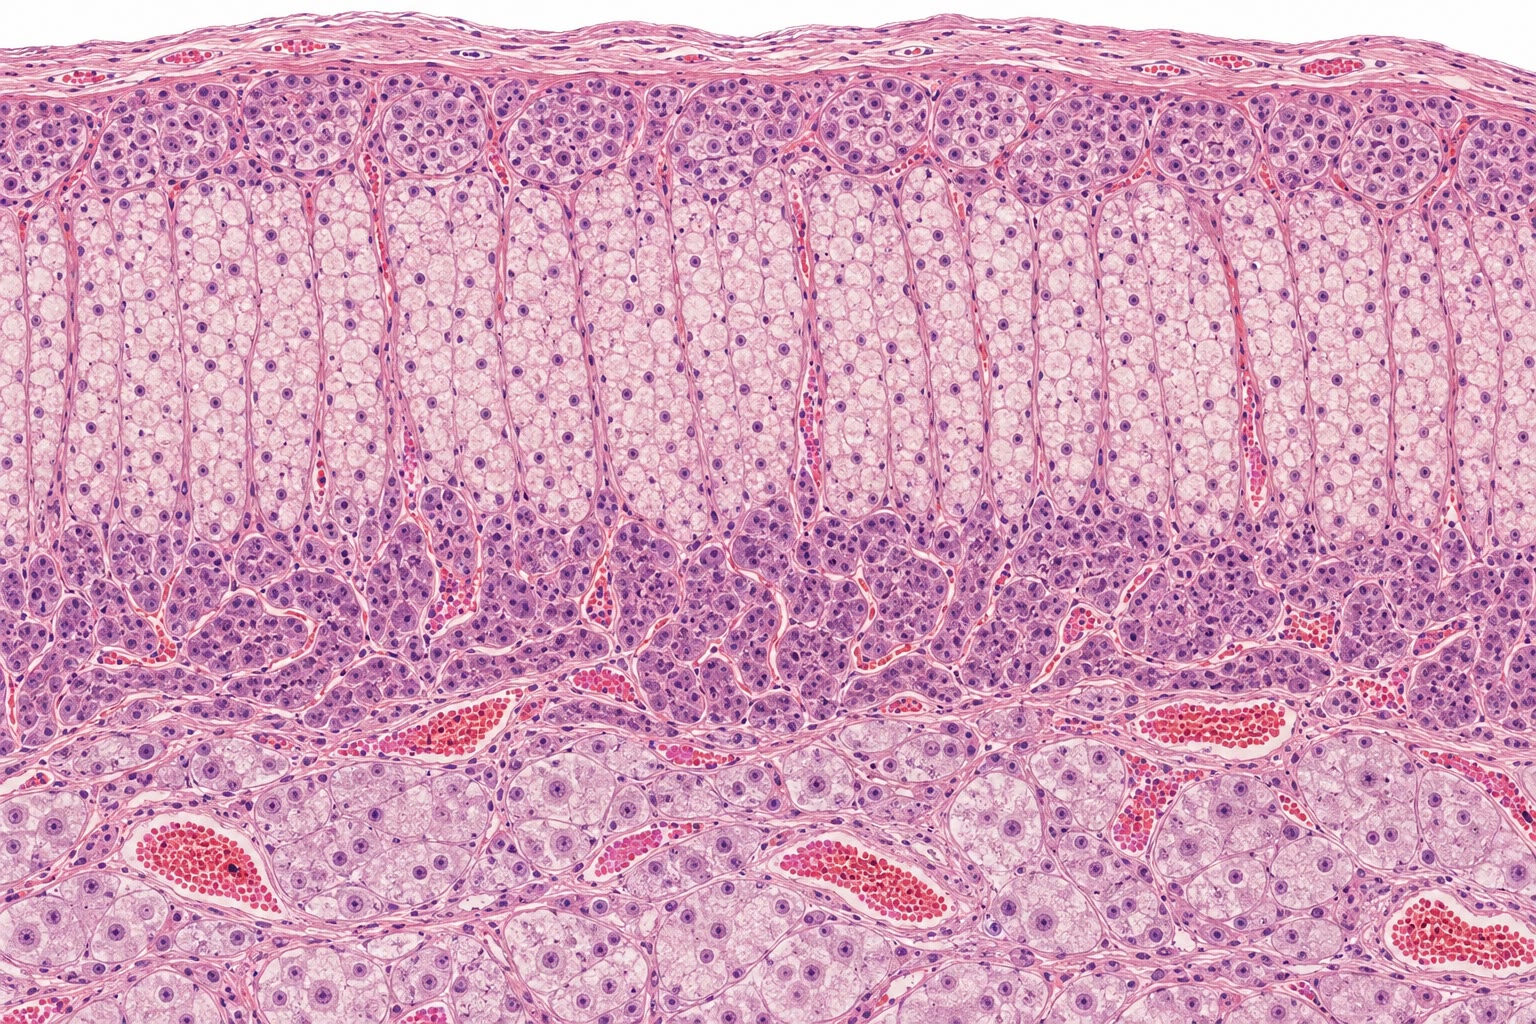
\includegraphics[width=0.5\linewidth]{images/book5/ai/b5-21-adrenal-section.jpg}\hspace{0.04\linewidth}
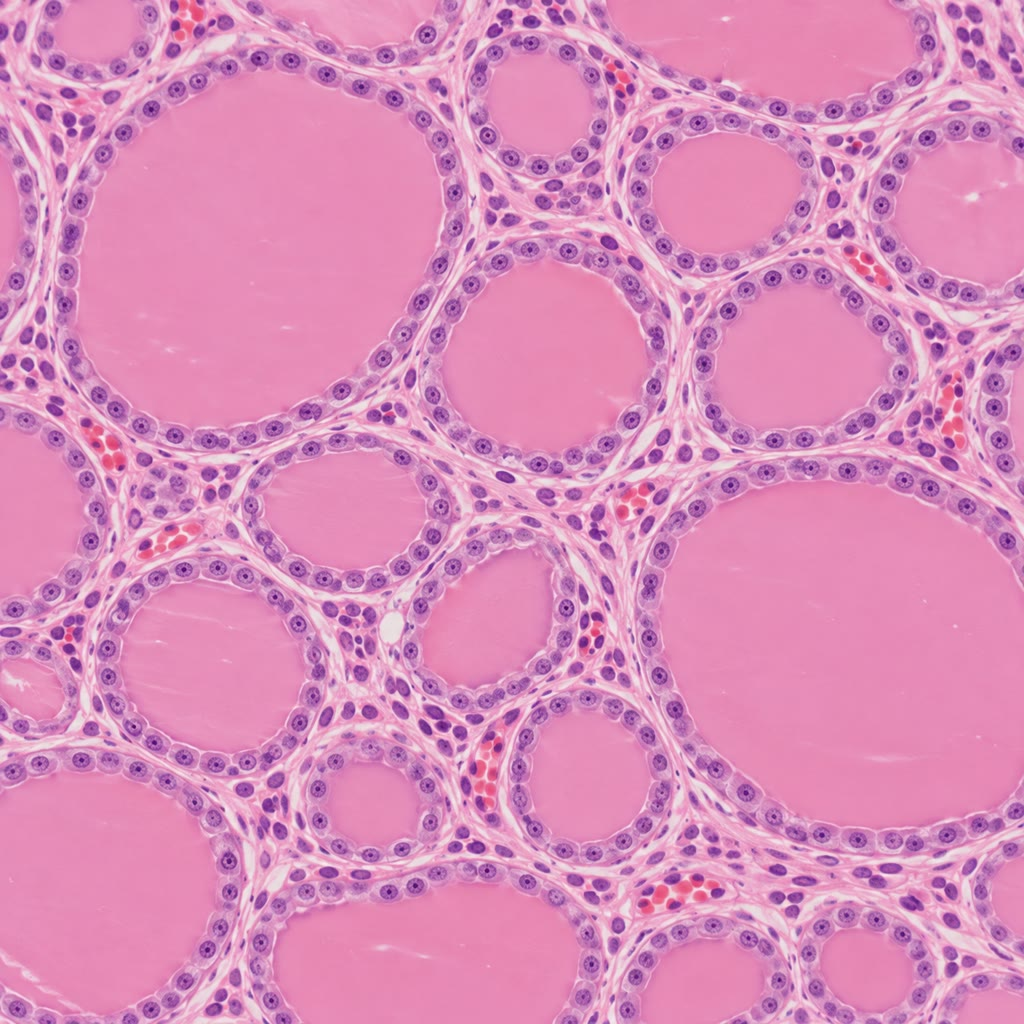
\includegraphics[width=0.36\linewidth]{images/book5/ai/b5-21-thyroid-follicles.jpg}

{\small À esquerda: a glândula adrenal em corte --- o córtex em suas três
zonas (\omterm{def:b3:renal-osmoregulation:controls}{aldosterona} na mais externa, cortisol na ampla zona média,
androgênios na mais interna) em torno de uma medula de células
cromafins secretoras de adrenalina, que é, por origem, um \omterm{def:b3:nervous-systems:comparative}{gânglio}
simpático. À direita: folículos tireoidianos, cada um uma esfera de
células em volta de um estoque de coloide com meses de \omterm{def:b3:endocrinology:hormone}{hormônio} ligado à
tireoglobulina.}
\end{omfigure}

\section{A glicose: a alça mais apertada}

\begin{definition}[Insulina e glucagon]\label{def:b3:endocrinology:glucose}
\index{insulina}\index{glucagon}\index{ilhota de Langerhans}\index{GLUT4}\index{diabetes melito}
O sangue contém cerca de \qty{5}{g} de glicose, a \qty{5}{mmol/L}
(\qty{90}{mg/dL}), e o encéfalo queima \qty{120}{g} por dia e não
consegue queimar outra coisa; uma refeição entrega \qty{75}{g} em uma
hora. As \emph{ilhotas de Langerhans}, um milhão de agrupamentos de
alguns milhares de células espalhados pelo pâncreas, guardam a alça. As
células $\beta$ percebem a glicose metabolizando-a: mais glicose, mais
ATP, fechamento de um canal de potássio sensível a ATP, despolarização,
entrada de cálcio e exocitose de \emph{insulina}, um \omterm{def:b3:endocrinology:hormone}{hormônio peptídico}
clivado de um precursor único. A insulina diz ao músculo e à gordura que
levem o transportador \emph{GLUT4} às suas superfícies e captem glicose,
ao fígado que armazene glicose como glicogênio e pare de produzi-la, e à
gordura que pare de liberar ácidos graxos: é o \omterm{def:b3:endocrinology:hormone}{hormônio} do estado
alimentado, o único que baixa a glicose sanguínea. As células $\alpha$
liberam \emph{glucagon} quando a glicose cai: o fígado degrada glicogênio
e faz glicose nova a partir de aminoácidos e lactato. A adrenalina, o
cortisol e o \omterm{def:b3:endocrinology:hormone}{hormônio} do crescimento também elevam a glicose, e a
redundância não é simétrica: um corpo pode se defender de uma queda por
quatro vias e de uma elevação por uma. O \emph{diabetes melito} é a
falência dessa uma: o tipo 1, a destruição autoimune das células $\beta$,
precisa de insulina desde o primeiro dia; o tipo 2, nove casos em dez,
começa como resistência dos tecidos à insulina, compensada por anos com
mais insulina, até que as células $\beta$ não deem conta e a glicose
suba.
\end{definition}

\begin{theorem}[A alça insulina--glicose]\label{thm:b3:endocrinology:loop}
\index{ganho de alça}\index{ponto de ajuste}\index{oscilação amortecida}
Escreva $g$ e $i$ para os desvios da glicose e da \omterm{def:b3:endocrinology:glucose}{insulina} plasmáticas
em relação a seus valores de jejum. A glicose é depurada a uma taxa
proporcional ao próprio excesso (a efetividade da glicose $a$) e ao
excesso de \omterm{def:b3:endocrinology:glucose}{insulina} (sensibilidade $s$); a \omterm{def:b3:endocrinology:glucose}{insulina} é secretada em
proporção ao excesso de glicose ($\beta$) e depurada à taxa $\gamma$;
entra uma carga $u$:
\[
\dot g = -a\,g - s\,i + u, \qquad \dot i = \beta\,g - \gamma\,i .
\]
Sob uma carga constante $u$ a glicose se estabiliza em
\[
g^{*} = \frac{u}{a}\cdot\frac{1}{1 + L}, \qquad L = \frac{s\beta}{a\gamma},
\]
de modo que a retroalimentação divide a perturbação que um corpo não
regulado sofreria por $1 + L$, o \emph{\omterm{thm:b3:endocrinology:loop}{ganho de alça}} mais um. Depois de
um bolus o retorno é governado pelos autovalores
$\lambda = -\tfrac{a + \gamma}{2} \pm \sqrt{\tfrac{(a+\gamma)^{2}}{4} - (a\gamma + s\beta)}$:
monótono se $s\beta < (a - \gamma)^{2}/4$, e, caso contrário, uma
\omterm{thm:b3:endocrinology:loop}{oscilação amortecida} de frequência angular $\omega = \sqrt{a\gamma + s\beta -
(a+\gamma)^{2}/4}$ decaindo como $\mathrm{e}^{-(a+\gamma)t/2}$
--- a glicose passa abaixo de seu valor de jejum antes de se acomodar,
que é a hipoglicemia leve duas ou três horas depois de uma refeição
açucarada. A resistência à \omterm{def:b3:endocrinology:glucose}{insulina} baixa $s$: o estado estacionário de
jejum sob a própria produção hepática do corpo sobe, e a alça compensa
com um $i^{*}$ mais alto até que o $\beta$ das células $\beta$ também
caia, quando a compensação falha.
\end{theorem}
\begin{proof}
Regime estacionário: $\dot i = 0$ dá $i^{*} = \beta g^{*}/\gamma$; pondo
isso em $\dot g = 0$: $a g^{*} + s\beta g^{*}/\gamma = u$, donde $g^{*} =
u/(a + s\beta/\gamma) = (u/a)/(1 + L)$. Dinâmica: a matriz do sistema é
$\begin{pmatrix} -a & -s\\ \beta & -\gamma\end{pmatrix}$, com traço
$-(a+\gamma)$ e determinante $a\gamma + s\beta$; sua equação
característica $\lambda^{2} + (a+\gamma)\lambda + (a\gamma + s\beta) = 0$
tem as raízes indicadas. As duas têm parte real negativa, de modo que o
estado de jejum é estável; as raízes são complexas quando o
discriminante $(a+\gamma)^{2}
- 4(a\gamma + s\beta) = (a-\gamma)^{2} - 4s\beta$ é negativo, a condição dada, e então $g(t) = \mathrm{e}^{-(a+\gamma)t/2}(A\cos\omega t
+ B\sin\omega t)$, que cruza o
zero. Resistência: com $u$ a produção basal do fígado e $s$ reduzida, $L$
cai e $g^{*}$ sobe para o mesmo $u$; $i^{*} = \beta g^{*}/\gamma$ sobe
junto (hiperinsulinemia); se $\beta$ então cair, $L$ cai mais ainda e
$g^{*}$ escala rumo a $u/a$.
\end{proof}

\begin{omfigure}
\begin{tikzpicture}
\begin{axis}[
  width=0.58\linewidth, height=5.6cm,
  axis x line=bottom, axis y line=left,
  xmin=0, xmax=180, ymin=40, ymax=200,
  xlabel={minutos após um bolus de glicose}, ylabel={glicose plasmática (mg/dL)},
  xlabel style={font=\small, at={(axis description cs:0.5,-0.12)}, anchor=north}, ylabel style={font=\small},
  tick label style={font=\small}, xtick={0,30,60,90,120,150,180}, ytick={60,90,120,150,180},
  clip=false,
]
\addplot[very thick, omDef, smooth] coordinates {(0,190) (6,165) (12,131) (18,102) (24,84) (30,77) (36,78) (42,82) (48,86) (54,89) (60,91) (66,92) (72,91) (78,91) (84,90) (90,90) (96,90) (102,90) (108,90) (114,90) (120,90) (126,90) (132,90) (138,90) (144,90) (150,90) (156,90) (162,90) (168,90) (174,90) (180,90)};
\draw[dashed, gray] (axis cs:0,90) -- (axis cs:180,90);
\node[font=\scriptsize, gray, anchor=south east] at (axis cs:180,91) {nível de jejum};
\node[font=\scriptsize, omDef, anchor=west, align=left] at (axis cs:75,150) {modelo: $a = \qty{0.02}{min^{-1}}$, $\gamma = \qty{0.1}{min^{-1}}$,\\$s\beta = \qty{0.01}{min^{-2}}$, ganho de alça $L = 5$;\\mínimo em \qty{32}{min}, período \qty{68}{min}};
\node[font=\scriptsize, omThm, anchor=north] at (axis cs:24,70) {queda abaixo do jejum};
\end{axis}
\begin{axis}[
  at={(0.6\linewidth,0)}, anchor=south west,
  width=0.33\linewidth, height=5.6cm,
  axis x line=bottom, axis y line=left,
  xmin=0, xmax=180, ymin=0, ymax=40,
  xlabel={minutos}, ylabel={insulina (mU/L)},
  xlabel style={font=\small, at={(axis description cs:0.5,-0.12)}, anchor=north}, ylabel style={font=\small},
  tick label style={font=\small}, xtick={0,60,120,180}, ytick={0,10,20,30,40},
]
\addplot[very thick, omProp, smooth] coordinates {(0,10.0) (6,30.0) (12,33.7) (18,28.5) (24,20.4) (30,13.4) (36,8.9) (42,7.1) (48,7.1) (54,7.9) (60,9.0) (66,9.8) (72,10.2) (78,10.4) (84,10.4) (90,10.2) (96,10.1) (102,10.0) (108,10.0) (114,9.9) (120,10.0) (126,10.0) (132,10.0) (138,10.0) (144,10.0) (150,10.0) (156,10.0) (162,10.0) (168,10.0) (174,10.0) (180,10.0)};
\draw[dashed, gray] (axis cs:0,10) -- (axis cs:180,10);
\end{axis}
\end{tikzpicture}

{\small A alça linear depois de um bolus que eleva a glicose em
\qty{100}{mg/dL}. A \omterm{def:b3:endocrinology:glucose}{insulina} atinge o pico em dez minutos e a glicose
volta à linha de base em vinte, e então cai abaixo dela; uma
retroalimentação forte que age por um \omterm{def:b3:endocrinology:hormone}{hormônio} com seu próprio tempo de
depuração retorna como uma \omterm{thm:b3:endocrinology:loop}{oscilação amortecida}, e não como um simples
decaimento.}
\end{omfigure}

\begin{proof}[Evidência]
Von Mering e Minkowski (1889) removeram o pâncreas de um cão e
produziram diabetes --- as moscas que se juntavam em sua urina
denunciavam o açúcar; ligar os ductos, o que destruía o tecido digestivo
mas poupava as ilhotas, não produzia. Banting e Best (1921), com a
purificação de Collip, extraíram o princípio das ilhotas e baixaram o
açúcar sanguíneo de um cão diabético, e depois o de Leonard Thompson
(janeiro de 1922). Sanger sequenciou a \omterm{def:b3:endocrinology:glucose}{insulina} (1955), a primeira
sequência de uma proteína; Yalow e Berson a mediram no sangue (1959) e
descobriram que os diabéticos de início adulto tinham, a princípio, mais
\omterm{def:b3:endocrinology:glucose}{insulina} que os sadios --- resistência, e não deficiência. As bactérias
da Genentech fizeram \omterm{def:b3:endocrinology:glucose}{insulina} humana em 1978, o primeiro fármaco
recombinante.
\end{proof}

\begin{omfigure}
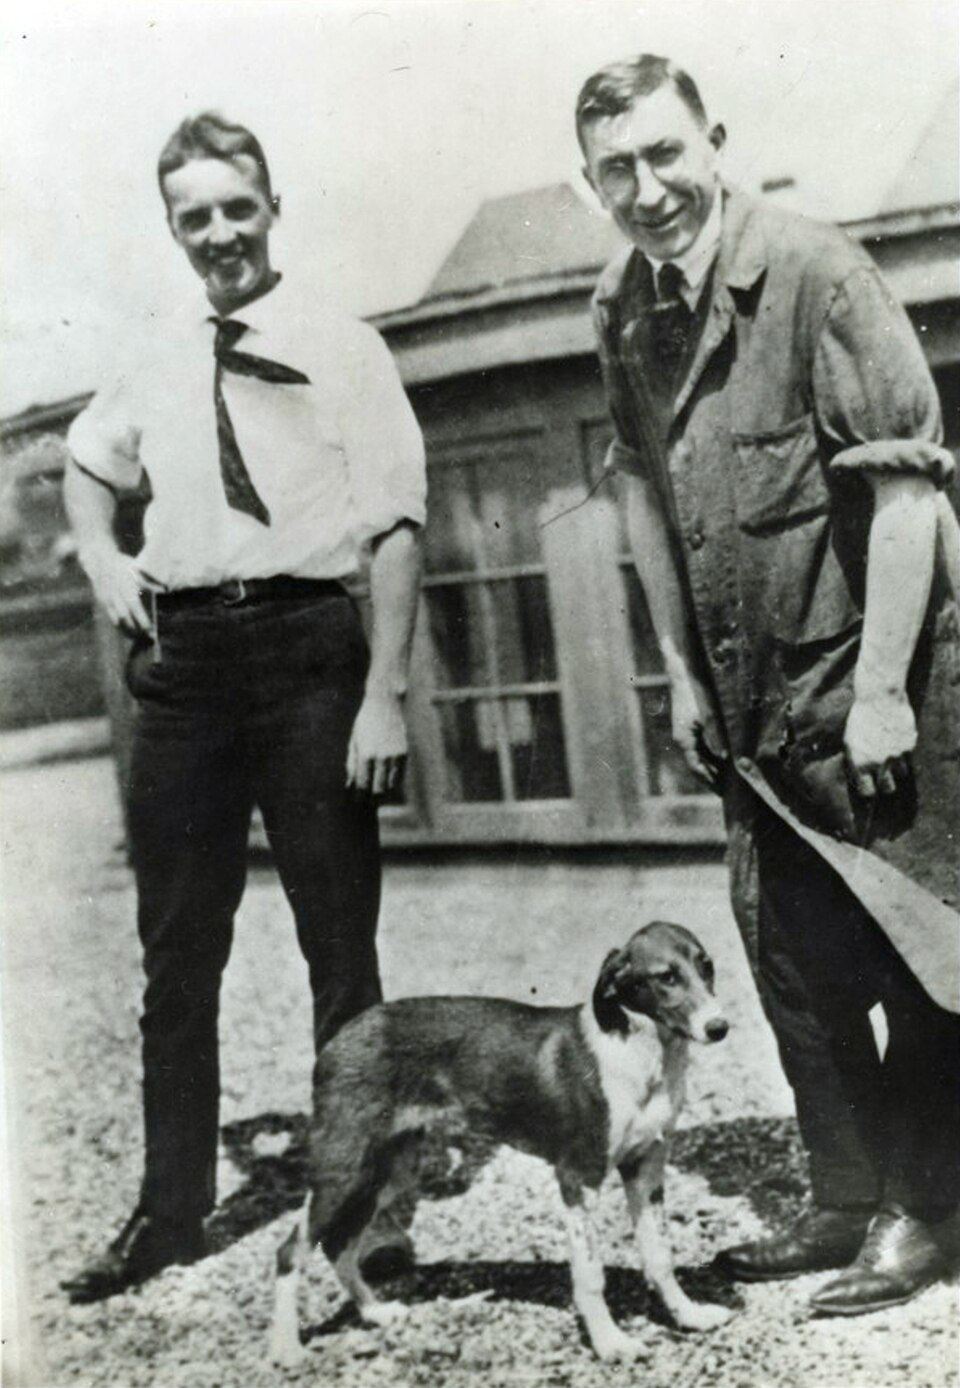
\includegraphics[width=0.42\linewidth]{images/book5/banting-best.jpg}\hspace{0.04\linewidth}
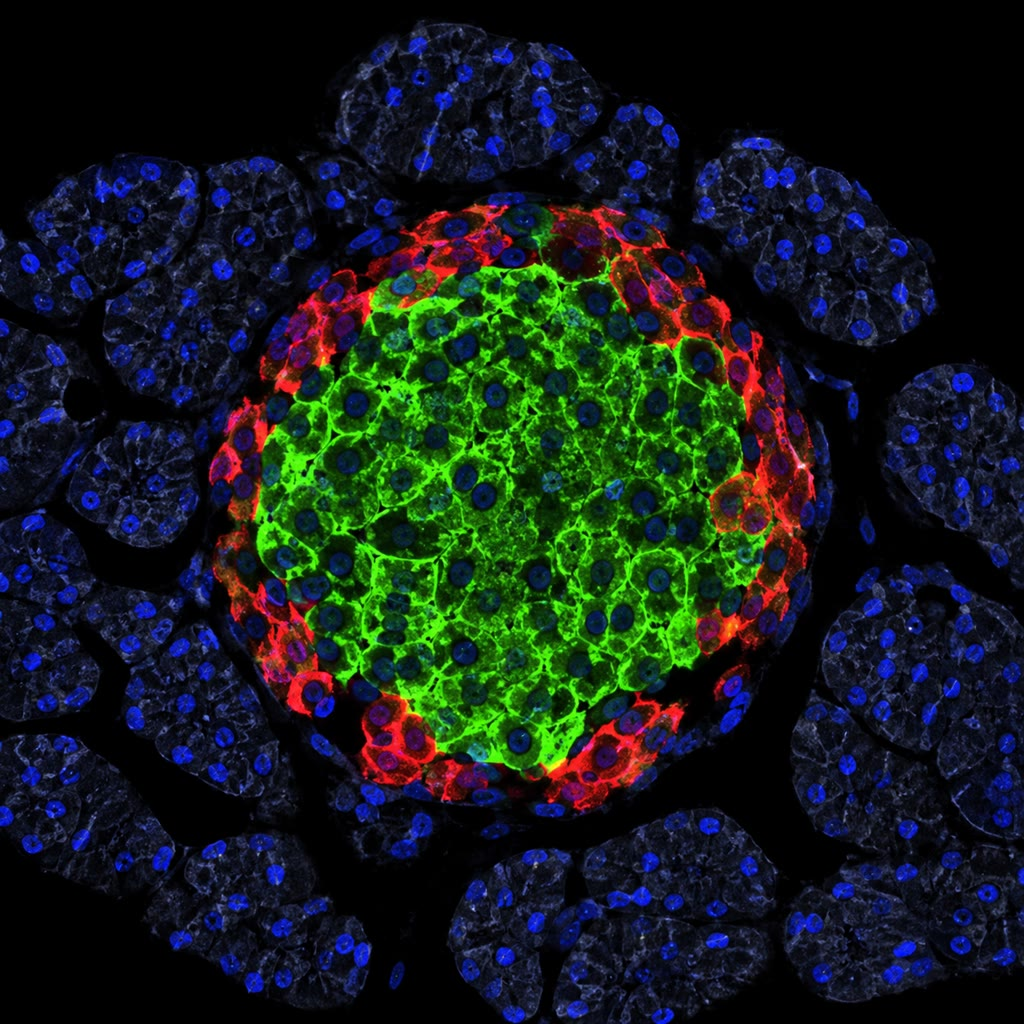
\includegraphics[width=0.42\linewidth]{images/book5/ai/b5-21-pancreatic-islet.jpg}

{\small À esquerda: Frederick Banting e Charles Best no telhado do
prédio da faculdade de medicina em Toronto, por volta de 1924, com um
dos cães dos experimentos da \omterm{def:b3:endocrinology:glucose}{insulina} (fotografia em domínio público). À
direita: uma \omterm{def:b3:endocrinology:glucose}{ilhota de Langerhans}, com células $\beta$ produtoras de
\omterm{def:b3:endocrinology:glucose}{insulina} no centro e células $\alpha$ de \omterm{def:b3:endocrinology:glucose}{glucagon} na borda, num mar de
ácinos exócrinos.}
\end{omfigure}

\begin{method}[Ler a alça da glicose num paciente]\label{met:b3:endocrinology:ogtt}
\index{teste de tolerância à glicose}\index{HbA1c}
(1) Glicose plasmática de jejum: normal abaixo de \qty{5.6}{mmol/L},
diabetes em \qty{7.0}{mmol/L} ou acima em duas ocasiões. (2) Teste oral
de tolerância à glicose: \qty{75}{g} de glicose bebidos; a glicose
plasmática em duas horas é normal abaixo de \qty{7.8}{mmol/L}, e
diabetes em \qty{11.1}{mmol/L} ou acima --- o valor de duas horas lê o
ganho da alça; o de jejum, seu \omterm{thm:b3:endocrinology:loop}{ponto de ajuste}. (3) Hemoglobina glicada,
a \emph{HbA1c}: a glicose se prende irreversivelmente à hemoglobina a
uma taxa proporcional à sua concentração, e as hemácias vivem 120 dias,
de modo que a fração glicada integra a glicose média dos últimos três
meses sem jejum --- normal abaixo de \qty{5.7}{\%}, diabetes a partir de
\qty{6.5}{\%}. (4) Para separar resistência de deficiência, meça a
\omterm{def:b3:endocrinology:glucose}{insulina} (ou seu subproduto, o peptídeo~C) ao lado: \omterm{def:b3:endocrinology:glucose}{insulina} alta com
glicose alta é resistência; peptídeo~C ausente é tipo~1.
\end{method}

\section{O cálcio, e o relógio}

\begin{definition}[Homeostase do cálcio]\label{def:b3:endocrinology:calcium}
\index{paratormônio}\index{calcitriol}\index{vitamina D}\index{osteoporose}
O cálcio ionizado do plasma é mantido em \qty{1.2}{mmol/L} dentro de
alguns por cento, porque ele fixa a excitabilidade de todo nervo e todo
músculo: baixo demais e eles disparam espontaneamente (tetania), alto
demais e ficam lentos. As quatro glândulas paratireoides o percebem com
um receptor de superfície e secretam \emph{paratormônio} (PTH) ao longo
de uma sigmoide inversa e íngreme: o PTH mobiliza cálcio do osso, faz o
rim reabsorvê-lo e excretar fosfato, e ativa a \emph{vitamina D} ---
feita na pele pela luz ultravioleta ou ingerida, hidroxilada no fígado e
depois no rim a \emph{calcitriol} ---, que faz o intestino absorver
cálcio. O osso é o reservatório, um quilograma de cálcio, remodelado
continuamente por osteoclastos e osteoblastos sob o PTH, o calcitriol, o
estrógeno e a carga. A carência de vitamina D dá raquitismo nas crianças
e ossos moles nos adultos; a queda do estrógeno na menopausa inclina o
remodelamento para a reabsorção e dá \emph{osteoporose}; um adenoma de
paratireoide eleva o cálcio, dissolve o osso e forma cálculos renais ---
``ossos, pedras, gemidos e lamentos''.
\end{definition}

\begin{definition}[O relógio circadiano]\label{def:b3:endocrinology:clock}
\index{relógio circadiano}\index{núcleo supraquiasmático}\index{genes do relógio}\index{melatonina}\index{zeitgeber}
Quase toda célula carrega um \emph{relógio circadiano}: uma alça de
transcrição e tradução em que as proteínas CLOCK e BMAL1 ligam os genes
\emph{Per} e \emph{Cry}, cujas proteínas se acumulam, entram no núcleo
depois de um atraso de horas e reprimem sua própria transcrição, e então
são degradadas, liberando a repressão --- um ciclo em cerca de vinte e
quatro horas, fixado pelas taxas do atraso e da degradação. Os relógios
do corpo são sincronizados por um relógio-mestre de vinte mil neurônios
do \emph{núcleo supraquiasmático} do \omterm{def:b3:endocrinology:axes}{hipotálamo}, que é ele próprio
acertado pela luz através de uma classe dedicada de \omterm{def:b3:sensory-systems:retina}{células ganglionares}
da \omterm{def:b3:sensory-systems:retina}{retina} (que contêm melanopsina, e não os pigmentos dos \omterm{def:b3:sensory-systems:retina}{bastonetes} ou
dos \omterm{def:b3:sensory-systems:retina}{cones}), e que sinaliza a noite ao corpo pela \emph{melatonina} da
pineal, secretada apenas no escuro. O relógio agenda o cortisol antes de
acordar, a temperatura corporal mais baixa às 4 da manhã, o \omterm{def:b3:endocrinology:hormone}{hormônio} do
crescimento no primeiro sono, a sensibilidade à \omterm{def:b3:endocrinology:glucose}{insulina} mais alta pela
manhã; comida, exercício e temperatura são \emph{zeitgebers} secundários
que podem puxar os relógios periféricos para longe do central, que é o
mal-estar do trabalhador em turnos e do jet lag --- um relógio do fígado
num horário e um do encéfalo em outro.
\end{definition}

\begin{proof}[Evidência]
Konopka e Benzer (1971) rastrearam moscas mutantes em busca de ritmos
alterados de emergência e encontraram três alelos de um gene, o
\emph{period}: um dia curto (19 h), um dia longo (29 h) e nenhum ritmo
--- um relógio com período genético. Hardin, Hall e Rosbash (1990)
descobriram que o mRNA e a proteína de \emph{period} oscilam com um
atraso entre si, e que a proteína reprime seu próprio gene: a alça.
Ralph e Menaker (1990) transplantaram o \omterm{def:b3:endocrinology:clock}{núcleo supraquiasmático} de um
hamster mutante com ritmo de 20 horas para um hamster normal cujo
próprio núcleo havia sido destruído: o receptor passou a rodar em 20
horas --- o período pertencia ao tecido transplantado. Em humanos
mantidos num bunker sem pistas de tempo o ritmo correu livre num pouco
mais de 24 horas; uma luz forte à noite o atrasava, e de manhã o
adiantava.
\end{proof}

\begin{omfigure}
\begin{tikzpicture}[every node/.style={font=\scriptsize}, >=stealth]
  \node[draw, thick, rounded corners, fill=omDef!20, align=center] (cb) at (0,1.6) {ativadores\\CLOCK--BMAL1};
  \node[draw, thick, rounded corners, fill=omProp!25, align=center] (pc) at (3.6,1.6) {\emph{Per}, \emph{Cry}\\transcritos};
  \node[draw, thick, rounded corners, fill=omThm!20, align=center] (pr) at (3.6,-0.4) {proteínas PER, CRY\\acumulam, dimerizam};
  \node[draw, thick, rounded corners, fill=omMeth!25, align=center] (nu) at (0,-0.4) {entram no núcleo\\depois de horas};
  \draw[->, thick] (cb) -- (pc) node[midway, above, font=\tiny] {ativam};
  \draw[->, thick] (pc) -- (pr) node[midway, right, font=\tiny] {tradução, atraso};
  \draw[->, thick] (pr) -- (nu);
  \draw[-|, thick, omThm] (nu) -- (cb) node[midway, left, font=\tiny, omThm, align=right] {reprimem\\seus próprios\\ativadores};
  \draw[->, thick, gray] (nu.south) -- ++(0,-0.5) node[below, font=\tiny, gray] {degradadas: repressão cessa, ciclo recomeça $\approx$ \qty{24}{h}};
  % right: daily profile
  \begin{scope}[shift={(7.2,-1.6)}]
    \draw[->] (0,0) -- (5.6,0) node[right, font=\tiny] {hora};
    \draw[->] (0,0) -- (0,3.4);
    \foreach \x/\l in {0/0, 1.4/6, 2.8/12, 4.2/18, 5.6/24} { \draw (\x,0) -- (\x,-0.08) node[below, font=\tiny] {\l}; }
    \fill[gray!25] (0,0) rectangle (1.4,3.4); \fill[gray!25] (5.1,0) rectangle (5.6,3.4);
    \node[font=\tiny, gray!60!black] at (0.7,3.2) {noite};
    \draw[very thick, omMeth!70!black, domain=0:5.6, samples=60, smooth, variable=\x] plot (\x, {1.6 + 1.2*cos(deg(2*3.1416*(\x-1.9)/5.6))});
    \node[font=\tiny, omMeth!70!black] at (3.1,3.1) {cortisol: pico às 8 h};
    \draw[very thick, omDef, domain=0:5.6, samples=60, smooth, variable=\x] plot (\x, {0.9 + 0.7*cos(deg(2*3.1416*(\x-0.7)/5.6))});
    \node[font=\tiny, omDef] at (2.7,0.18) {melatonina: à noite};
  \end{scope}
\end{tikzpicture}

{\small À esquerda: o núcleo do relógio molecular, uma alça de
\omterm{def:b3:endocrinology:axes}{retroalimentação negativa} com um atraso de horas, que é o que uma alça
precisa ter para oscilar em vez de se acomodar. À direita: dois
\omterm{def:b3:endocrinology:hormone}{hormônios} que ele agenda --- o cortisol subindo antes do amanhecer para
preparar o dia, a \omterm{def:b3:endocrinology:clock}{melatonina} marcando a noite.}
\end{omfigure}

\begin{remark}[A homeostase como controle]\label{rem:b3:endocrinology:control}
Toda alça deste capítulo tem as mesmas peças: um sensor (o metabolismo
da célula $\beta$, o receptor de cálcio da paratireoide, o receptor de
\omterm{prop:b3:endocrinology:thyroid}{hormônio tireoidiano} da \omterm{def:b3:endocrinology:axes}{hipófise}), um controlador que compara com um
\omterm{thm:b3:endocrinology:loop}{ponto de ajuste}, um \omterm{def:b3:endocrinology:hormone}{hormônio} efetor com sua própria meia-vida e uma
retroalimentação que reduz o erro por um fator $1 + L$, mas nunca a
zero. O que difere é a temporização --- segundos para a adrenalina, uma
hora para a \omterm{def:b3:endocrinology:glucose}{insulina}, dias para a tiroxina, uma vida para o osso --- e o
preço do compromisso: uma alça rápida com um efetor atrasado oscila; uma
alça lenta deixa uma perturbação persistir. A clínica vê as alças de
fora, pelos pares que a retroalimentação acopla: um TSH alto com uma
T$_{4}$ baixa é uma glândula falha, um TSH alto com uma T$_{4}$ alta é
uma \omterm{def:b3:endocrinology:axes}{hipófise} falha; uma \omterm{def:b3:endocrinology:glucose}{insulina} alta com uma glicose alta é
resistência, uma \omterm{def:b3:endocrinology:glucose}{insulina} baixa com uma glicose alta é destruição. Para
ler o nível de um \omterm{def:b3:endocrinology:hormone}{hormônio} é preciso sempre perguntar o que seu
comandante estava fazendo.
\end{remark}

\section{Exercícios}

\begin{exercise}[$\star$]\label{exo:b3:endocrinology:1}
Classifique a \omterm{def:b3:endocrinology:glucose}{insulina}, o cortisol, a adrenalina, a tiroxina e a
vasopressina por química, localização do receptor, rapidez de ação e
meia-vida.
\end{exercise}

\begin{exercise}[$\star$]\label{exo:b3:endocrinology:2}
Desenhe o eixo tireoidiano com sua retroalimentação e preveja o TSH e a
T$_{4}$ em: uma tireoide destruída; um \omterm{def:b3:cancer-biology:hallmarks}{tumor} hipofisário secretor de
TSH; um paciente tomando tiroxina demais; carência de iodo.
\end{exercise}

\begin{exercise}[$\star$]\label{exo:b3:endocrinology:3}
Por que um corpo tem quatro \omterm{def:b3:endocrinology:hormone}{hormônios} que elevam a glicose sanguínea e
apenas um que a baixa? O que isso prevê sobre os perigos relativos de
\omterm{def:b3:endocrinology:glucose}{insulina} demais e de \omterm{def:b3:endocrinology:glucose}{insulina} de menos?
\end{exercise}

\begin{exercise}[$\star$]\label{exo:b3:endocrinology:4}
O que é um \omterm{def:b3:endocrinology:clock}{zeitgeber}? Dê três, diga qual deles o relógio-mestre usa e
explique o que acontece com um viajante que cruza oito fusos horários.
\end{exercise}

\begin{exercise}[$\star\star$]\label{exo:b3:endocrinology:5}
Uma célula tem \num{20000} receptores com $K_{d} = \qty{1}{nM}$ e
responde ao máximo quando \num{500} estão ocupados. Encontre a
EC$_{50}$. Depois de uma semana de \omterm{def:b3:endocrinology:hormone}{hormônio} alto a célula tem \num{2000}
receptores: nova EC$_{50}$? Interprete para a resistência à \omterm{def:b3:endocrinology:glucose}{insulina}.
\end{exercise}

\begin{exercise}[$\star\star$]\label{exo:b3:endocrinology:6}
Com $\kappa = \qty{0.46}{L/pmol}$ e um TSH normal de \qty{1.5}{mU/L} com
T$_{4}$ livre de \qty{15}{pmol/L}, calcule o TSH quando a T$_{4}$ for
$13$, $11$, $9$ e \qty{25}{pmol/L}. Em qual desses casos a T$_{4}$ ainda
estaria dentro de uma faixa de referência de
\qtyrange{10}{20}{pmol/L} enquanto o TSH está fora de
\qtyrange{0.4}{4}{mU/L}?
\end{exercise}

\begin{exercise}[$\star\star$]\label{exo:b3:endocrinology:7}
Na alça do \cref{thm:b3:endocrinology:loop} com $a = \qty{0.02}{min^{-1}}$,
$\gamma = \qty{0.1}{min^{-1}}$, $\beta = \qty{0.05}{mU\,L^{-1}\,min^{-1}}$
por mg/dL e $s = \qty{0.2}{mg\,dL^{-1}\,min^{-1}}$ por mU/L, calcule o
\omterm{thm:b3:endocrinology:loop}{ganho de alça}, o excesso estacionário de glicose sob uma carga constante
de \qty{2}{mg/dL/min}, o mesmo sem retroalimentação, e o excesso
estacionário de \omterm{def:b3:endocrinology:glucose}{insulina}.
\end{exercise}

\begin{exercise}[$\star\star$]\label{exo:b3:endocrinology:8}
Mesmos parâmetros: o retorno depois de um bolus é oscilatório? Calcule o
período e o tempo para a amplitude cair por $\mathrm{e}$. Agora reduza
$s$ à metade (resistência à \omterm{def:b3:endocrinology:glucose}{insulina}): recalcule os dois e o novo \omterm{thm:b3:endocrinology:loop}{ganho
de alça}.
\end{exercise}

\begin{exercise}[$\star\star$]\label{exo:b3:endocrinology:9}
A meia-vida do cortisol é de \qty{80}{min}. Um paciente que tomou
\qty{40}{mg} de prednisolona por dia durante um ano para de repente.
Explique, nível por nível, por que ele pode entrar em colapso com uma
infecção leve três dias depois, e o que o eixo mostraria se fosse medido
(ACTH, cortisol, resposta ao ACTH injetado).
\end{exercise}

\begin{exercise}[$\star\star\star$]\label{exo:b3:endocrinology:10}
Mostre que uma \omterm{def:b3:endocrinology:axes}{retroalimentação negativa} de uma variável $\dot x = f(x)$
com $f' < 0$ não pode oscilar, enquanto a alça de duas variáveis do
teorema pode, e explique em palavras por que o relógio precisa de um
atraso de horas entre a transcrição e a repressão para produzir um
período de 24 horas. O que aconteceria com o período se a PER fosse
degradada duas vezes mais depressa?
\end{exercise}

\begin{exercise}[$\star\star\star$]\label{exo:b3:endocrinology:11}
O \omterm{def:b3:endocrinology:calcium}{paratormônio} segue $\text{PTH} = P_{\max}/(1 +
\mathrm{e}^{k(\text{Ca} - \text{Ca}_{0})})$ com $\text{Ca}_{0} =
\qty{1.2}{mmol/L}$ e $k = \qty{20}{L/mmol}$. Calcule o PTH como fração do
máximo em Ca $= 1.10$, $1.15$, $1.20$, $1.25$ e \qty{1.30}{mmol/L}, a
inclinação no \omterm{thm:b3:endocrinology:loop}{ponto de ajuste}, e explique por que tamanha inclinação é
desejável para o cálcio mas seria perigosa para a glicose.
\end{exercise}

\begin{exercise}[$\star\star\star$]\label{exo:b3:endocrinology:12}
A glicose se prende à hemoglobina a uma taxa $k\,G$ por unidade de
tempo, com $k$ tal que uma glicose média de \qty{5.5}{mmol/L} dê
\qty{5}{\%} de glicação ao longo dos 120 dias de vida de uma hemácia.
Deduza a HbA1c em função da glicose média, o valor a \qty{10}{mmol/L}, e
explique por que um paciente com anemia hemolítica (hemácias vivendo 60
dias) tem uma HbA1c enganosamente baixa.
\end{exercise}

\section{Problema: O Açúcar no Sangue}

\begin{problem}[{Problema de fim de semana --- um \omterm{met:b3:endocrinology:ogtt}{teste de tolerância à
glicose} lido pela alça linear insulina--glicose: a distribuição de uma
dose de \qty{75}{g}, o \omterm{thm:b3:endocrinology:loop}{ganho de alça} e o retorno amortecido, o que a
resistência e a falência das células $\beta$ fazem ao \omterm{thm:b3:endocrinology:loop}{ponto de ajuste} de
jejum, um diagnóstico a partir dos números e o eixo tireoidiano ao lado,
terminando no \omterm{thm:b3:endocrinology:loop}{ganho de alça}, no tempo de retorno e na glicose de jejum
da alça que falha}]
\label{pb:b3:endocrinology:1}
Dados: um adulto sadio, volume de distribuição da glicose \qty{15}{L},
glicose de jejum \qty{90}{mg/dL} (\qty{5}{mmol/L}), \omterm{def:b3:endocrinology:glucose}{insulina} de jejum
\qty{10}{mU/L}. Parâmetros da alça: $a = \qty{0.02}{min^{-1}}$, $\gamma =
\qty{0.1}{min^{-1}}$, $\beta = 0.05$ (mU/L por min por mg/dL), $s = 0.2$
(mg/dL por min por mU/L). Produção hepática basal de glicose $u_{0} =
\qty{2}{mg/dL/min}$ (já equilibrada no estado de jejum pela eliminação
de jejum). Uma dose oral de \qty{75}{g} é absorvida ao longo de uma
hora. Tireoide: $\text{TSH} = 1.5\,\mathrm{e}^{-0.46(T_{4} - 15)}$ mU/L.
Massa molar da glicose \qty{180}{g/mol}.

\medskip
\noindent\textbf{Parte I --- A dose.}
\begin{enumerate}
  \item Expresse a glicose de jejum em mmol/L e confira a conversão a
        partir de mg/dL. Quantos gramas de glicose há no volume de
        distribuição em jejum?
  \item Se as \qty{75}{g} inteiras aparecessem de uma vez em \qty{15}{L},
        de quanto a glicose subiria (mg/dL e mmol/L)? Por que o pico
        real, cerca de \qty{60}{mg/dL} acima do jejum, fica tão aquém?
  \item Absorvida ao longo de \qty{60}{min}, a dose entra a que taxa em
        mg/dL por minuto? Compare com $u_{0}$.
  \item Sem resposta alguma de \omterm{def:b3:endocrinology:glucose}{insulina} ($s = 0$), a glicose obedeceria a
        $\dot
        g = -a g + u$. Excesso estacionário sob a taxa de absorção,
        e a constante de tempo da aproximação. Onde estaria a glicose
        depois de uma hora?
  \item Com a alça, calcule $L$ e o excesso estacionário sob a mesma
        taxa. Compare com a questão~4.
  \item Explique por que o encéfalo é protegido dos dois lados: do que
        ele precisa, e o que glicose demais faz aos tecidos ao longo dos
        anos.
\end{enumerate}

\medskip
\noindent\textbf{Parte II --- O retorno.}
\begin{enumerate}[resume]
  \item Escreva a equação característica da alça e calcule o traço, o
        determinante e o discriminante.
  \item Calcule $\omega$ e o período da \omterm{thm:b3:endocrinology:loop}{oscilação amortecida}, e o tempo
        de decaimento $2/(a + \gamma)$.
  \item Partindo de um excesso de \qty{100}{mg/dL} com a \omterm{def:b3:endocrinology:glucose}{insulina} em seu
        valor de jejum, a solução é $g(t) = 100\,\mathrm{e}^{-0.06t}
        (\cos\omega t + c\sin\omega t)$. Encontre $c$ a partir de $\dot g(0) = -a\cdot
        100$.
  \item Quando a glicose volta pela primeira vez ao jejum (primeiro zero
        de $g$)? Estime a queda abaixo do jejum no primeiro mínimo.
  \item \omterm{def:b3:endocrinology:glucose}{Insulina}: $i(t)$ tem a mesma exponencial e a mesma frequência.
        Argumente, a partir de $\dot i = \beta g - \gamma i$, que seu
        pico vem depois que a glicose começou a cair e antes que a
        glicose chegue ao jejum.
  \item Por que um teste de tolerância real, com absorção ao longo de uma
        hora em vez de um bolus, mostra um pico aos 30--60 minutos e um
        retorno em duas horas, e apenas uma queda leve às três?
\end{enumerate}

\medskip
\noindent\textbf{Parte III --- Quando a alça falha.}
\begin{enumerate}[resume]
  \item A resistência à \omterm{def:b3:endocrinology:glucose}{insulina} reduz $s$ à metade. Novo $L$? O $u_{0}$
        do fígado é agora atendido por um novo estado estacionário de
        jejum: usando $g^{*} = (u_{0}/a)/(1
        + L)$ como o excesso sobre
        uma linha de base idealizada sem regulação, descubra de quanto a
        glicose de jejum sobe em relação ao estado sadio (calcule os dois
        valores de $g^{*}$ e subtraia).
  \item \omterm{def:b3:endocrinology:glucose}{Insulina} de jejum no estado resistente: calcule $i^{*} = \beta
        g^{*}/\gamma$ nos dois estados e a razão. Como a clínica chama
        isso?
  \item Agora as células $\beta$ falham: $\beta$ cai também para um
        quinto. Novo $L$, novo excesso de jejum. Converta para mmol/L e
        compare com o limiar diabético de \qty{7}{mmol/L}.
  \item O retorno ainda é oscilatório no estado da questão~15? Calcule o
        discriminante e a constante de tempo do modo mais lento.
  \item Um paciente tem glicose de jejum de \qty{8}{mmol/L}, \omterm{def:b3:endocrinology:glucose}{insulina} de
        jejum de \qty{30}{mU/L} e valor de duas horas de \qty{13}{mmol/L}.
        Diagnostique o tipo e o mecanismo a partir dos pares.
  \item Outro tem glicose de jejum de \qty{15}{mmol/L}, peptídeo~C
        indetectável, e perdeu \qty{8}{kg} em dois meses. Diagnostique, e
        explique a perda de peso em termos do que os tecidos fazem sem
        \omterm{def:b3:endocrinology:glucose}{insulina}.
  \item HbA1c: se a glicose média do primeiro paciente é \qty{9}{mmol/L},
        e \qty{5.5}{mmol/L} dão \qty{5}{\%}, estime sua HbA1c supondo
        proporcionalidade.
\end{enumerate}

\medskip
\noindent\textbf{Parte IV --- A glândula ao lado.}
\begin{enumerate}[resume]
  \item A T$_{4}$ livre é \qty{12}{pmol/L}. Calcule o TSH. A T$_{4}$ está
        na faixa de \qtyrange{10}{20}{pmol/L}? O TSH está em
        \qtyrange{0.4}{4}{mU/L}? Como se chama esse estado?
  \item A T$_{4}$ é \qty{7}{pmol/L}: TSH? Um paciente com essa T$_{4}$
        mas um TSH de \qty{0.3}{mU/L}: onde está a lesão?
  \item A meia-vida da tiroxina é de \qty{7}{d}. Um paciente em
        reposição esquece uma semana de comprimidos. A que fração o nível
        cai, e por que a semana esquecida é menos perigosa que um dia
        esquecido de reposição de cortisol?
  \item Doença de Graves: um \omterm{def:b3:adaptive-immunity:antibody}{anticorpo} ocupa o receptor de TSH. Preveja a
        T$_{4}$, o TSH e o efeito da relação log-linear sobre o TSH
        medido.
  \item Explique num parágrafo por que o nível de um \omterm{def:b3:endocrinology:hormone}{hormônio} nada
        significa sem o nível de seu comandante, usando os quatro pares
        da última observação do capítulo.
  \item Resuma: o \omterm{thm:b3:endocrinology:loop}{ganho de alça} sadio (questão~5), o período e o tempo de
        decaimento do retorno (questão~8) e a glicose de jejum da alça
        que falha (questão~15).
\end{enumerate}
\end{problem}
